\begin{figure}[H]
  \centering
  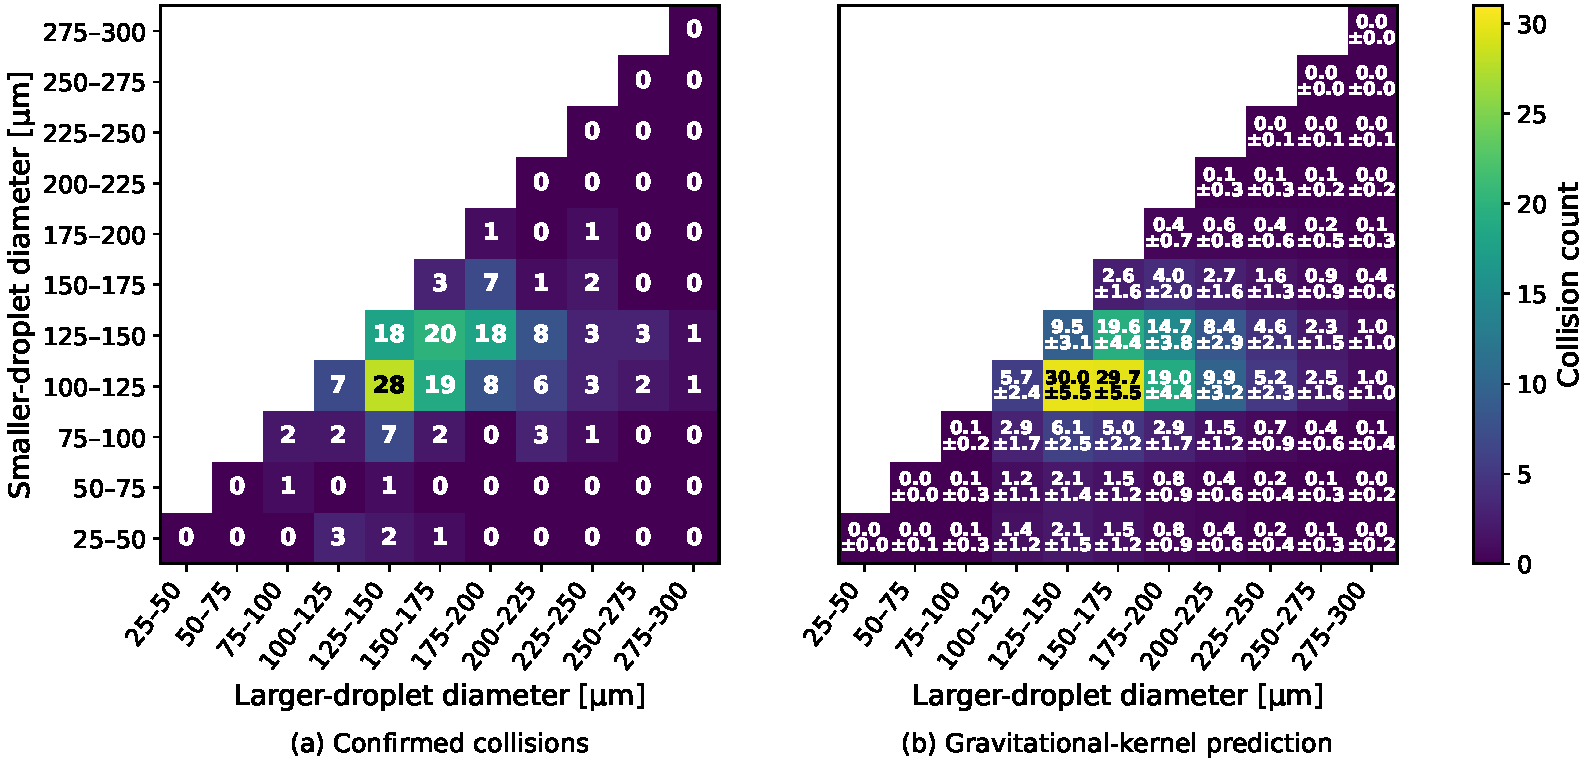
\includegraphics[width=\linewidth]{figures/expresult/collision_count_map_observed_vs_hall_260715.pdf}
  \caption{Parent-diameter-pair distributions of collision–coalescence counts pooled over the 14 experimental sequences. (a) Visually confirmed event counts. (b) Gravitational-kernel predictions using the experimentally measured number-density distributions. The horizontal and vertical axes represent the larger and smaller parent diameters, respectively, using \qty{25}{\micro\meter} bins over \(\qty{25}{\micro\meter}\leq D<\qty{300}{\micro\meter}\). Each unordered diameter-bin pair is counted once. Diagonal cells include droplets in the same diameter bin, not necessarily droplets of identical diameter. Cell annotations in (b) give the predicted count ±1 standard deviation, rounded to one decimal place.}
  \label{fig:experimental_collision_count_map}
\end{figure}
